\subsubsection{Spectrum}\label{sec:spectrum}
The spectrum tab shows spectra as a count histograms, retrieved from a connected detector or loaded from a compatible file. It can show several spectra combined in one plot or in separate tabs within the spectrum tab, see \autoref{fig:spectrum_with_cursor}. This can be changed under \texttt{Options -> Tabbed-/Combined Spectrum View} (then selecting the files or data to be shown).


Background spectra can be viewed as: \textit{Background overlay} and \textit{background subtract} or not at all: \textit{No background}. \textit{Background overlay} shows the background spectrum overlaid on top of the main (foreground) spectrum. \textit{Background subtract} subtracts the background, channel by channel, from the foreground spectrum. Note that this is a hard background subtraction and will thus effect spectrum ROI calculations. Both \textit{Background overlay} and \textit{Background subtract} are limited to show count rate values.

\begin{figure}[H]
    \centering
    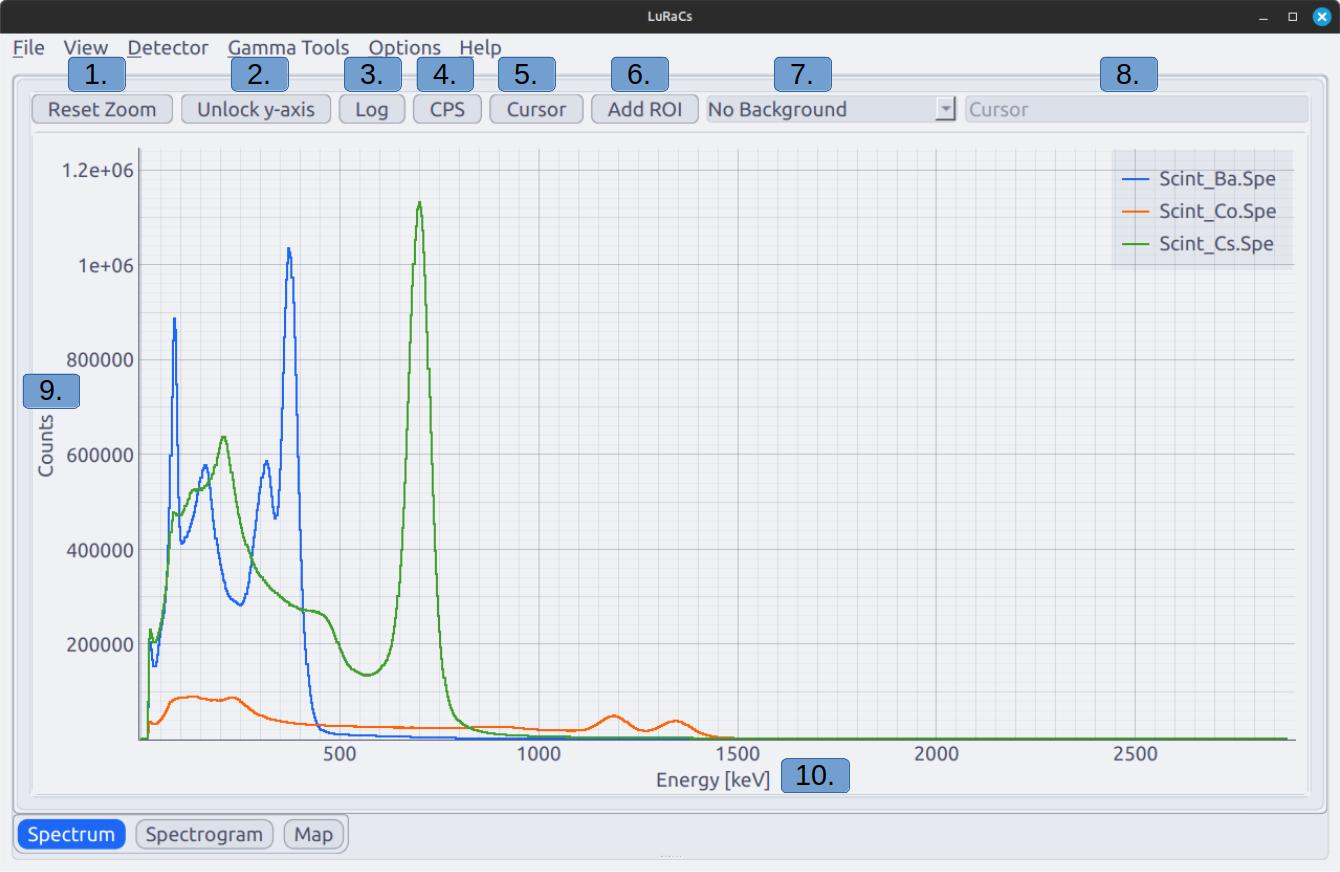
\includegraphics[width = .9\linewidth]{images/interface/spectrum_view.jpg}
    \caption{Spectra of Ba-133, C-60 and Cs-137 displayed in \textit{Combined Spectrum View}.}
    \label{fig:spectrum_view}
    \begin{flushleft}
        \begin{enumerate}
            \item \textbf{Rest Zoom} resets the zoom of the spectrum view and locks the y-axis if unlocked.
            \item \textbf{Unlock y-axis} allows the y-axis to be zoomed independently (by scrolling the wheel of the mouse) and disables autoscaling.
            \item \textbf{Log} set the scale of the y-axis to logarithmic or reset back to linear scale.
            \item \textbf{CPS} normalises the spectrum to the live time, or real time if live time is not available but real time is.
            \item \textbf{Cursor} toggles the spectrum cursor, see \autoref{fig:spectrum_with_cursor}.
            \item \textbf{Add ROI} adds a customisable \textit{region of interest} to the spectrum, see \autoref{fig:spectrum_with_roi}.
            \item Switch the use of background spectrum. Options are \textit{No background}, \textit{Background overlay} and \textit{background subtract}. See the section above.
            \item Display for info from the cursor, see \autoref{fig:spectrum_with_cursor}.
            \item The y-axis show either total counts or time normalised counts in units of \unit{\per\second}.
            \item The x-axis always display energy in units of keV.
        \end{enumerate}
    \end{flushleft}
\end{figure}

\textit{Regions of interest} (\textbf{ROI}) are sub regions of the spectrum bounded in energy and are useful in the analysis of spectrum peaks. Spectrum peaks can in most cases be approximated with a Gaussian function, knowing the function parameters is useful for many analyses. LuRaCs provides a method for fitting Gaussian functions to peaks inside ROIs and do so by default. These fits are required by other tools in the application. However, ROIs can also be configured to not perform fits. In these cases, only the total counts within each ROI are calculated.

\begin{figure}[H]
    \centering
    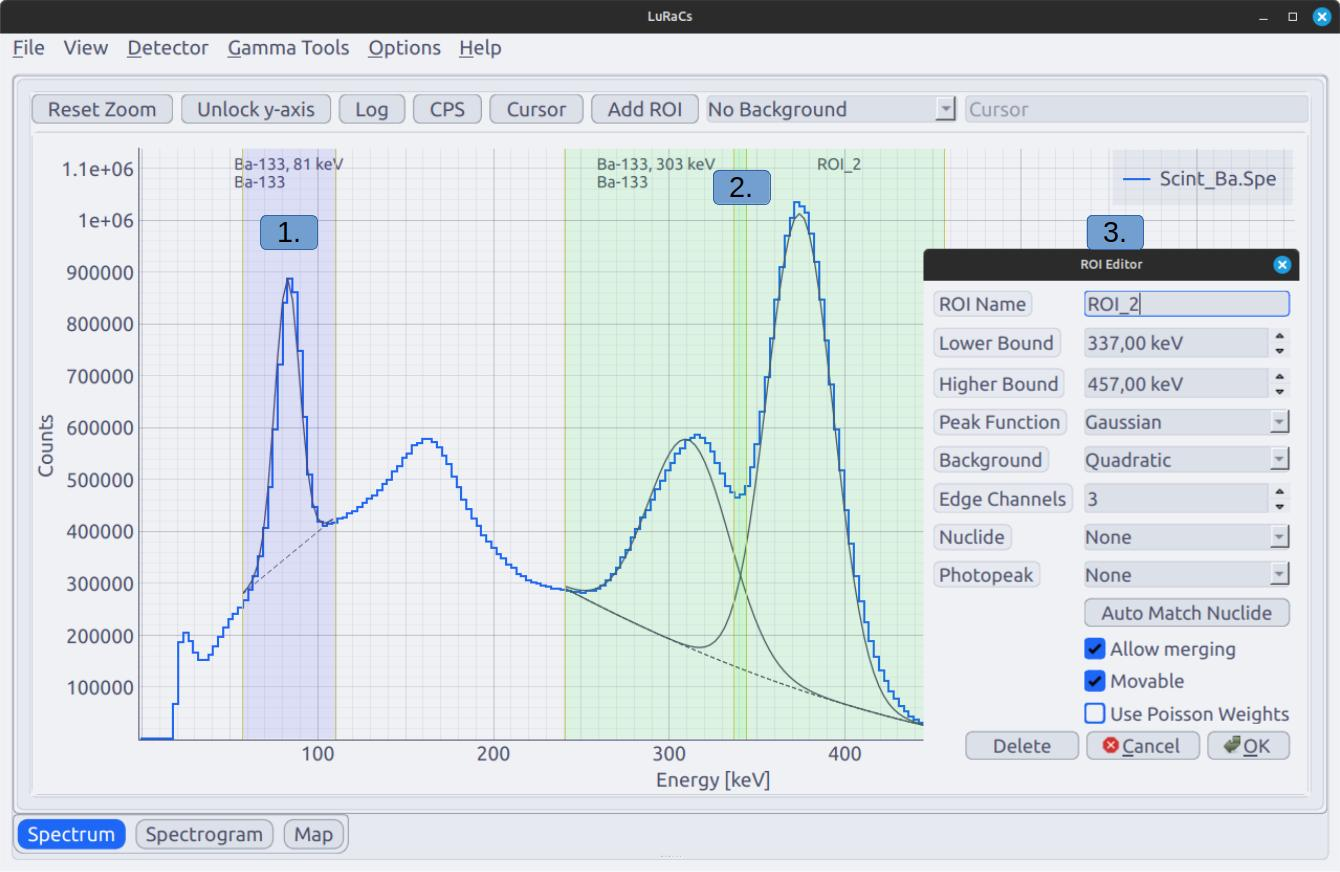
\includegraphics[width = .9\linewidth]{images/interface/spectrum_with_roi.jpg}
    \caption{A Ba-133 spectrum with three ROIs, two are merged and fitted to the same background. The ROI editor is open for the right most ROI (ROI\_2).}
    \label{fig:spectrum_with_roi}

    \begin{flushleft}
        \begin{enumerate}
            \item A ROI with one peak and a fitted Gaussian peak and linear background.
            \item Two merged ROIs that fit two Gaussian peaks on a shared quadratic background.
            \item The ROI editor for 'ROI\_2', see \autoref{tab:ROI_editor}.
        \end{enumerate}
    \end{flushleft}
\end{figure}

\begin{table}[H]
    \centering
    \caption{ROI Editor options}
    \label{tab:ROI_editor}
    \begin{tabular}{p{.3\textwidth}p{.7\textwidth}}
    \toprule
    \textbf{Field} & \textbf{Description} \\ \midrule
    ROI Name & An alias for the ROI used for display purposes and easier identification. \\
    Lower Bound & The lower energy bound of the ROI. \\
    Upper Bound & The upper energy bound of the ROI. \\
    Peak Function & The type of function fitted to the peak. Options are: \textit{Guassian}, \textit{None} \\
    Background & Type of function used as peak background. Options are: \textit{None}, \textit{Linear}, \textit{Quadratic} \\
    Edge Channels & The number of channels inside the ROI from the upper and lower bounds of the ROI used to fit the background. \\
    Nuclide & Assign a nuclide from the reference library to the ROI. Used for calculations by other tools. \\
    Photopeak & Choose the specific photon emission associated with the peak in the ROI. Options are based on the chosen nuclide. \\
    Auto Match Nuclide & Attempt to automatically find the nuclide and emission of the peak. If any nuclides are checked in the \textit{Isotopics}-tab, see section \ref{sec:isotopics}, the match is limited to these. Blind matches are often unreliable. \\
    Allow Merging & Allow the ROI to merge with other ROIs with merging allowed. \\
    Movable & If the ROI can be moved or its bounds adjusted by using the mouse. \\
    Use Poission Weights & Apply a 1/$\sigma$ weight to the optimisation to force the peak to emulate a Poission distribution. \\
    \bottomrule

    \end{tabular}
\end{table}

\begin{figure}[H]
    \centering
    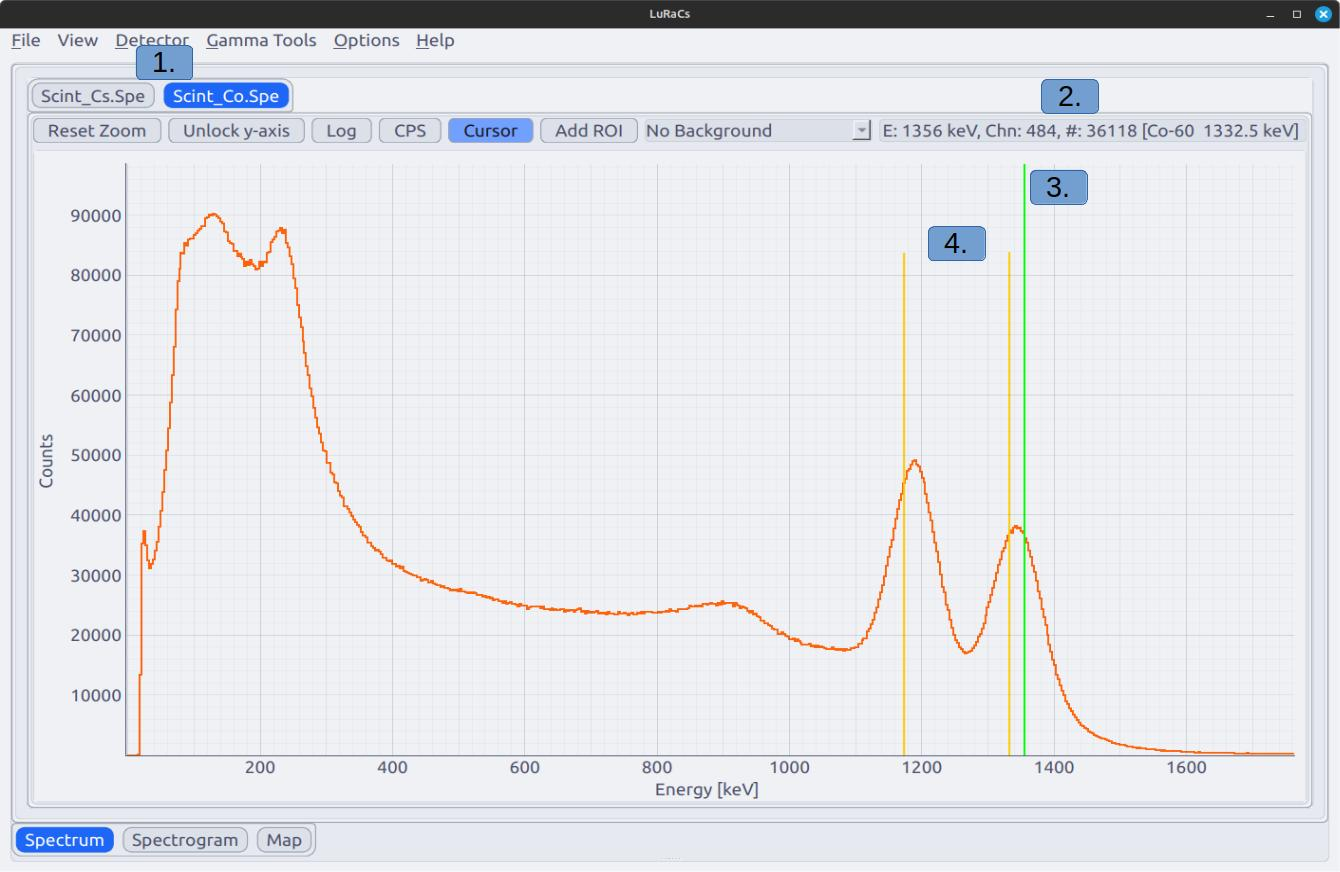
\includegraphics[width = .9\linewidth]{images/interface/spectrum_with_cursor.jpg}
    \caption{Co-60 spectrum with an active cursor.}
    \label{fig:spectrum_with_cursor}

    \begin{flushleft}
        \begin{enumerate}
            \item Tabs for selecting spectrum in \textit{Tabbed Spectrum View}.
            \item Spectrum information at the position of the cursor, showing of the corresponding energy and channels number, the number of counts in the channel, closest reference emission line as [\textit{nuclide} \textit{Emission Energy} \textit{Decay chain if applicable}]. Channel and channel counts are only displayed in tabbed spectrum view.
            \item Cursor in the spectrum.
            \item These always appear for the emission closest to the cursor in energy and does not weigh intensity or anything else. This can be disabled by \texttt{View -> Spectrum -> Show Cursor Emissions}.
        \end{enumerate}
    \end{flushleft}
\end{figure}